\section{Security and Privacy Analysis}
\label{sec:analysis}

As account uniqueness has been analyzed in Section \ref{subsec:overview},
in this section we prove security (i.e., user identification and RP designation) and privacy (i.e., IdP untraceability and RP unlinkability) of UPPRESSO.


\subsection{Adversarial Scenarios}

According to our design goals %(i.e., the desired security and privacy guarantees)
 and the potential adversaries listed in Section \ref{subsec:threatmodel}, we consider three adversarial scenarios as below
 and the security and privacy guarantees are proved against different adversaries.


%\noindent\textbf{Impersonation and identity injection against security.}
Security (i.e., user identification and RP designation) is proved against \emph{malicious RPs and users}.
 Malicious RPs and users could collude \cite{FettKS14,BrowserID,SPRESSO},
  attempting to (\emph{a}) impersonate an honest user to log into some honest RP
   or (\emph{b}) entice an honest user to log into an honest RP under another's account.
%These attacks break security of SSO services.

Provided that the security properties of UPPRESSO are satisfied,
    we analyze the privacy properties \emph{only} for successful logins
    because no meaningful account is derived in an unsuccessful login
where the initiating user or the target RP deviates from the specifications.
It makes no sense to track login activities resulting in meaningless accounts.
Therefore,
    an \emph{honest-but-curious} is considered in the proof of IdP untraceability,
while RP unlinkability is analyzed against \emph{honest-but-colluding} RPs and users
 which follow the protocols but share their information.

%\noindent\textbf{Login tracing by an IdP.}
%The honest-but-curious IdP tries to infer the identities of the RPs being visited by an honest user \cite{BrowserID, SPRESSO}.
%
%\noindent\textbf{Identity linkage by colluding RPs.}
%Malicious RPs could collude with each other and even malicious users, attempting to link logins across these RPs initiated by honest users \cite{maler2008venn, FirefoxAccount}. 


% \subsection{The Dolev-Yao Style Model for UPPRESSO}
% \label{dy-model}

% We develop a Dolev-Yao style model \cite{BrowserID, SPRESSO, FettKS16, FettKS17} for UPPRESSO, referred to as the \emph{\dyu\ model}, to formalize the login flow of UPPRESSO.
% % Dolev-Yao style models abstract cryptographic concepts into an algebra of symbolic messages to discover structural flaws using simple formal logic. % which has been used in the formal analysis of SSO protocols such as OAuth 2.0 \cite{FettKS16} and OIDC \cite{FettKS17}.
% The model abstracts the entities in a web system, such as web servers and browsers, as atomic processes, %which communicate with each other through events. % such as HTTPS requests and responses.
% and defines scripting processes to formulate client-side scripts.
% %The script is dependently invoked by the browser to process the server-defined logic.%such as verifying $Certificate_{RP}$. %postmessage events; %atomic process <-> scripting process, communication. %Other events change self-trigger.
% The atomic processes of UPPRESSO include an IdP process, a finite set of web servers for honest RPs, a finite set of honest browsers, and a finite set of attacker processes that model malicious RPs and malicious users.
% A browser may invoke an honest IdP script and multiple RP scripts that could be honest or malicious.
% The processes communicate with each other through events such as HTTPS requests and responses,
% %Although the scripts coexist in the same browser, they are strictly separated.
% except that the scripting processes communicate with each other through \verb+postMessage+ which are modeled as transmitted-to-itself events of a browser process.
% %To clearly indicate the action of postMessage communication, we define it as the transmitting-to-itself event of the browser (which is not defined in SPRESSO).


% Applying the \dyu\ model, we trace the lifecycle of an identity token from its generation at the IdP to its acceptance at an RP, locate the places where $PID_U$, $PID_{RP}$, and other elements related to the identity token such as $t$ and $u$ are processed, and locate the places where $PK$ is transmitted and used in the IdP script.
% We confirm the following conclusions in the \dyu\ model:
% (\emph{a}) an identity token binding pseudo-identities of honest entities, cannot be leaked to any malicious process;
% (\emph{b}) pseudo-identities and other elements in verified identity tokens cannot be manipulated by any malicious process;
% (\emph{c}) the IdP's public key set in the IdP script cannot be replaced or tampered with by any malicious process, within an honest browser;
% (\emph{d}) the IdP receives nothing about $t$ shared between two honest processes;
% (\emph{e}) $r$ is not leaked to any malicious process as it never leaves the IdP;
% and (\emph{f}) the RPs cannot receive anything about $u$ shared between two honest processes.


\subsection{Security}
\label{analysis-security}

In secure SSO systems, an identity token denoted as $TK$, which is requested by a user to visit an RP,
    \emph{enables only this user to log into only the honest target RP as her account at this RP}. It makes no sense to discuss the login results at malicious RPs.
$TK$ is signed by the IdP to bind $PID_{RP}$ and $PID_U$,
where (\emph{a}) the RP with $ID_{RP}$ is designated if $PID_{RP} = [t]ID_{RP}$ is calculated
    and (\emph{b}) $PID_U = [ID_U]PID_{RP}$ is calculated based on the initiating user's identity $ID_U$.

When authenticity, confidentiality and integrity of identity tokens are ensured, we summarize the following sufficient conditions of secure SSO services \cite{FettKS14,BrowserID,SPRESSO}:

\noindent \textbf{User Identification.} %At the designated RP, $TK$ identifies only the user who requests this identity token from the IdP. That is, 
From $TK$ the designated honest RP derives \emph{only} the meaningful account belonging to the user requesting $TK$.

\noindent \textbf{RP Designation.} From $TK$, \emph{only} the designated honest RP derives meaningful accounts.

%We prove that identity tokens in UPPRESSO and the enclosed pseudo-identities satisfy four properties, namely, \emph{RP designation}, \emph{user identification}, \emph{token confidentiality}, and \emph{token integrity}, which together ensure the security of UPPRESSO in the first adversarial scenario.

User identification and RP designation are proved in Theorems \ref{thm-u-id} and \ref{thm-rp-designation}, respectively.
As mentioned in Section \ref{implementations}, an (honest) RP directly derives accounts based on any signed identity token, without checking whether $PID_{RP}$ in the token is equal to $[t]ID_{RP}$ or not.
So we do not assume any relationship among $t$, $ID_{RP}$ and $PID_{RP}$ in the proofs.
Moreover,
the proofs assume \emph{malicious RPs colluding with users},
                which attempt to break the security guarantees of UPPRESSO,
by arbitrarily manipulating $t$ and/or sending $TK$ to an RP not designated.
% That is, even an unmatching token manipulated by malicious adversaries, does not break security of UPPRESSO.
% These properties are defined and proved specially for the proposed identity transformations in UPPRESSO, while checking $ID_{RP}$ in identity tokens by an RP is \emph{necessary} in other SSO solutions \cite{OpenIDConnect,BrowserID,SPRESSO,NIST2017draft,POIDC,save-flow,miso}.

Let's assume totally $s$ users and $p$ RPs in UPPRESSO,
    whose identities are denoted as $\mathbbm{ID}_U = \mathbbm{u} = \{u_{i; 1 \leq i \leq s}\}$ and $\mathbbm{ID}_{RP} = \{[r_{j;1 \leq j \leq p}]G\}$, respectively.
There are meaningful accounts $Acct_{i,j}=[u_i]ID_{RP_j} = [u_i r_j]G$ at each RP.
$Acct_{i,j}$ and $ID_{RP_j}$ are publicly-known, while $u_{i}$ and $r_{j}$ are kept unknown to adversaries.


%\vspace{-0.5mm}
%Because $TK$ works only at the ``implicitly'' designated RP and no meaningful user will be derived at any other RPs, % when $u_i$ and $r_j$ are kept unknown to adversaries,
% in Step 4.2 an RP does not check whether $PID_{RP}$ in the received token equals to $[t]ID_{RP}$ or not.

%\vspace{-0.5mm}

We prove user identification by showing that,
    at any RP designated by $TK$,
        a meaningless account not belonging to the initiating user will never be derived.

\begin{thm}[User Identification] Given unknown $\mathbbm{ID}_U$ and known $\mathbbm{A}cct$,
for any known $ID_{RP} \in \mathbbm{ID}_{RP}$, 
     malicious adversaries cannot find $\check{t}$ and $TK$ binding $PID_{RP} = \mathcal{F}_{PID_{RP}}(ID_{RP}, \hat{t})$
     and $PID_{\hat{U}}=\mathcal{F}_{PID_U}(ID_{\hat{U}}, PID_{RP})$ satisfying that $\mathcal{F}_{Acct}(PID_{\hat{U}}, \check{t}) = \mathcal{F}_{Acct\ast}(ID_{\check{U}}, ID_{RP})$, where $ID_{\hat{U}} \neq ID_{\check{U}}$ and $ID_{\hat{U}},ID_{\check{U}} \in \mathbbm{ID}_U$.
\label{thm-u-id}
\end{thm}
%\vspace{-0.5mm}

\noindent\textbf{\textsc{Proof.}}
It requires that, for any $ID_{RP}$, adversaries cannot find $\hat{t}$ and $\check{t}$ satisfying that $\mathcal{F}_{Acct}(PID_{\hat{U}}, \check{t}) = [\check{t}^{-1}]PID_{\hat{U}} = [\check{t}^{-1}ID_{\hat{U}}]PID_{RP}
= [\check{t}^{-1}\hat{t}ID_{\hat{U}}]ID_{RP}
    = [ID_{\check{U}}]ID_{RP} = \mathcal{F}_{Acct\ast}(ID_{\check{U}}, ID_{RP})$,
where $ID_{\hat{U}} \neq ID_{\check{U}}$.

When $u_{i}$ and $r_{j}$ are kept unknown, this is equivalent to the elliptic curve discrete logarithm problem (ECDLP) of $\check{t}^{-1}\hat{t} = \log_{[\hat{u}r]G}{[\check{u}r]G}$.
\hfill $\square$
\vspace{1.5mm}

Next,
we prove RP designation by showing that,
    at any honest RPs other than the designated one, no meaningful account will be derived from $TK$.
   % under an adversarial scenario involving malicious adversaries.

%\emph{Given $u \in \mathbbm{u}$ and $ID_{RP} \in \mathbbm{ID}_{RP}$, from $TK$ binding $PID_{RP}=[t]ID_{RP}$ and $PID_U = [u]PID_{RP}$, an honest RP with ${ID_{RP'} \neq ID_{RP}}$ cannot derive any $Acct = [u']ID_{RP'}$ where $u' \in \mathbbm{u}$ and $ID_{RP'} \in \mathbbm{ID}_{RP}$.}\label{thm-rp-designation}

\begin{thm}[RP Designation]
Given known $\mathbbm{ID}_{RP}$, known $\mathbbm{A}cct$ and unknown $\mathbbm{ID}_U$,
 malicious adversaries cannot find ${j_1}$, ${j_2}$, ${i_1}$, ${i_2}$, $t_1$, and $t_2$ which satisfy that $\mathcal{F}_{Acct}(\mathcal{F}_{PID_U}(ID_{U_{i_1}}, PID_{RP}), t_2) = \mathcal{F}_{Acct\ast}(ID_{U_{i_2}}, ID_{RP_{j_2}})$,
where $PID_{RP}$ may be calculated as $\mathcal{F}_{PID_{RP}}(ID_{RP_{j_1}}, t_1)$
    or arbitrarily generated (i.e., $RP_{j_1}$ or no RP is designated),
    ${j_1} \neq {j_2}$, $1 \leq j_1, j_2 \leq p$, and $1 \leq i_1, i_2 \leq s$.
\label{thm-rp-designation}
\end{thm}
%\vspace{-0.5mm}

\noindent\textbf{\textsc{Proof.}} 
If adversaries could find ${j_1}$, ${j_2}$, ${i_1}$, ${i_2}$, $t_1$ and $t_2$ which satisfy that $[{t_2}^{-1}t_1ID_{U_{i_1}}]ID_{RP_{j_1}} = [ID_{U_{i_2}}]ID_{RP_{j_2}}$
 where ${j_1} \neq {j_2}$,
 the ECDLP of ${t_2}^{-1}t_1 = \log_{[{u_{i_1}}{r_{j_1}}]G}{[{u_{i_2}}{r_{j_2}}]G}$ would be solved.

Or, the adversaries attempt to find $PID_{RP}$, ${j_2}$, ${i_1}$, ${i_2}$ and $t_2$ satisfying that  $[{{t_2}^{-1}}ID_{U_{i_1}}]PID_{RP} = [ID_{U_{i_2}}]ID_{RP_{j_2}}$,
        but this cannot be solved due to unknown $ID_{U_{i}}$.
\hfill $\square$
%\vspace{1mm}

\subsection{Privacy against IdP-based Login Tracing}
\label{subsec:IdP-privacy}

The honest IdP would attempt to infer the visited RPs,
by collecting information from the identity-token requests.
It does not obtain any information about the target RP in a login (e.g., $ID_{RP}$, $Enpt_{RP}$ or $Cert_{RP}$), except the RP's ephemeral pseudo-identity $PID_{RP}$.

We prove that, $PID_{RP}$ is \emph{indistinguishable} from a random variable on $\mathbb{E}$ to the IdP,
    and then
 it cannot (\emph{a}) link multiple logins visiting an RP or (\emph{b}) distinguish a login initiated by a user to visit any RP from those logins visiting other RPs by this user. % based on $PID_{RP}$s in the identity-token requests.

% So UPPRESSO prevents the honest-but-curious IdP from tracing a user's login activities.

\vspace{-0.5mm}
\begin{thm}[IdP Untraceability]
\emph{The IdP cannot distinguish $PID_{RP} = [t]ID_{RP}$ from a random variable on $\mathbb{E}$, where $t$ is random in $\mathbb{Z}_n$ and kept unknown to the IdP.}\label{thm-idp-untraceability}
\end{thm}
\vspace{-0.5mm}

\noindent\textbf{\textsc{Proof.}}
%$\mathbb{E}$ is a finite cyclic group, and the number of points on $\mathbb{E}$ is $n$.
As $G$ is a generator on $\mathbb{E}$ of order $n$, $ID_{RP} = [r]G$ is also a generator of order $n$.
As $t$ is uniformly-random in $\mathbb{Z}_n$ and kept unknown, $PID_{RP} = [t]ID_{RP}$ is \emph{indistinguishable} from a point that is uniformly-random on $\mathbb{E}$. \hfill $\square$
\vspace{1.5mm}

\noarxiv{This property actually has been proved in the Hash(EC)DH OPRF \cite{oprf-proved,voprf-proved} as obliviousness, where the OPRF server works similarly to the IdP and learns nothing about a client's inputs or outputs of the evaluated pseudo-random function (i.e., $ID_{RP}$ or $Acct$ in UPPRESSO).}

\subsection{Privacy against RP-based Identity Linkage}
\label{subsec:RP-privacy}

RPs could collude with some users,
    attempting to infer the identities of honest users
    or link an honest user's accounts across these RPs.


In each login, an RP obtains \emph{only} a random number $t$ and an identity token enclosing $PID_{RP}$ and $PID_U$. From the token, it learns only an ephemeral pseudo-identity $PID_{U} = [{ID_U}]{PID_{RP}}$ of the initiating user, from which it derives a \emph{permanent} locally-unique identifier (or account) $Acct = [ID_U]ID_{RP}$.
It cannot directly calculate $ID_U$ from $PID_{U}$ or $Acct$ due to the ECDLP.
Next, in Theorem \ref{thm-rp-unlinkability} we prove that, even if RPs collude with each other and some users by sharing $PID_U$s and other information observed in all their logins,
they still cannot link any login visiting an RP by an honest user to any other logins visiting other colluding RPs by honest users.


With the trapdoor $t$, $PID_{RP}$ and $PID_U$ can be transformed into $ID_{RP}$ and $Acct$, respectively, and vice versa.
So we denote all the information that an RP learns in a login as a tuple $L =(ID_{RP}, t, Acct)=([r]G, t, [ur]G)$.

As $c$ RPs collude with each other, they create a shared view of all logins visiting any of them, denoted as $\mathbbm{L}$.
When they collude further with $v$ users, the logins initiated by these users are picked out of $\mathbbm{L}$ and linked together as
$\mathfrak{L}^m=\left \{ \begin{matrix}
L^m_{1,1},&L^m_{1,2},&\cdots,&L^m_{1,c}\\
L^m_{2,1},& L^m_{2,2},&\cdots,&L^m_{2,c}\\
\cdots,&\cdots,&L^m_{i,j},&\cdots\\
L^m_{v,1},&L^m_{v,2},&\cdots,&L^m_{v,c}
\end{matrix}\right\}$,
where $L^m_{i, j}=([r_j]G, t_{i,j}, [u_ir_j]G) \in \mathbbm{L}$ for $1 \le i \le v$ and $1 \le j \le c$. Any login in $\mathbbm{L}$ but not linked in $\mathfrak{L}^m$ is initiated by an honest user to visit one of the $c$ colluding RPs.

\begin{figure}[tb]
  \centering
  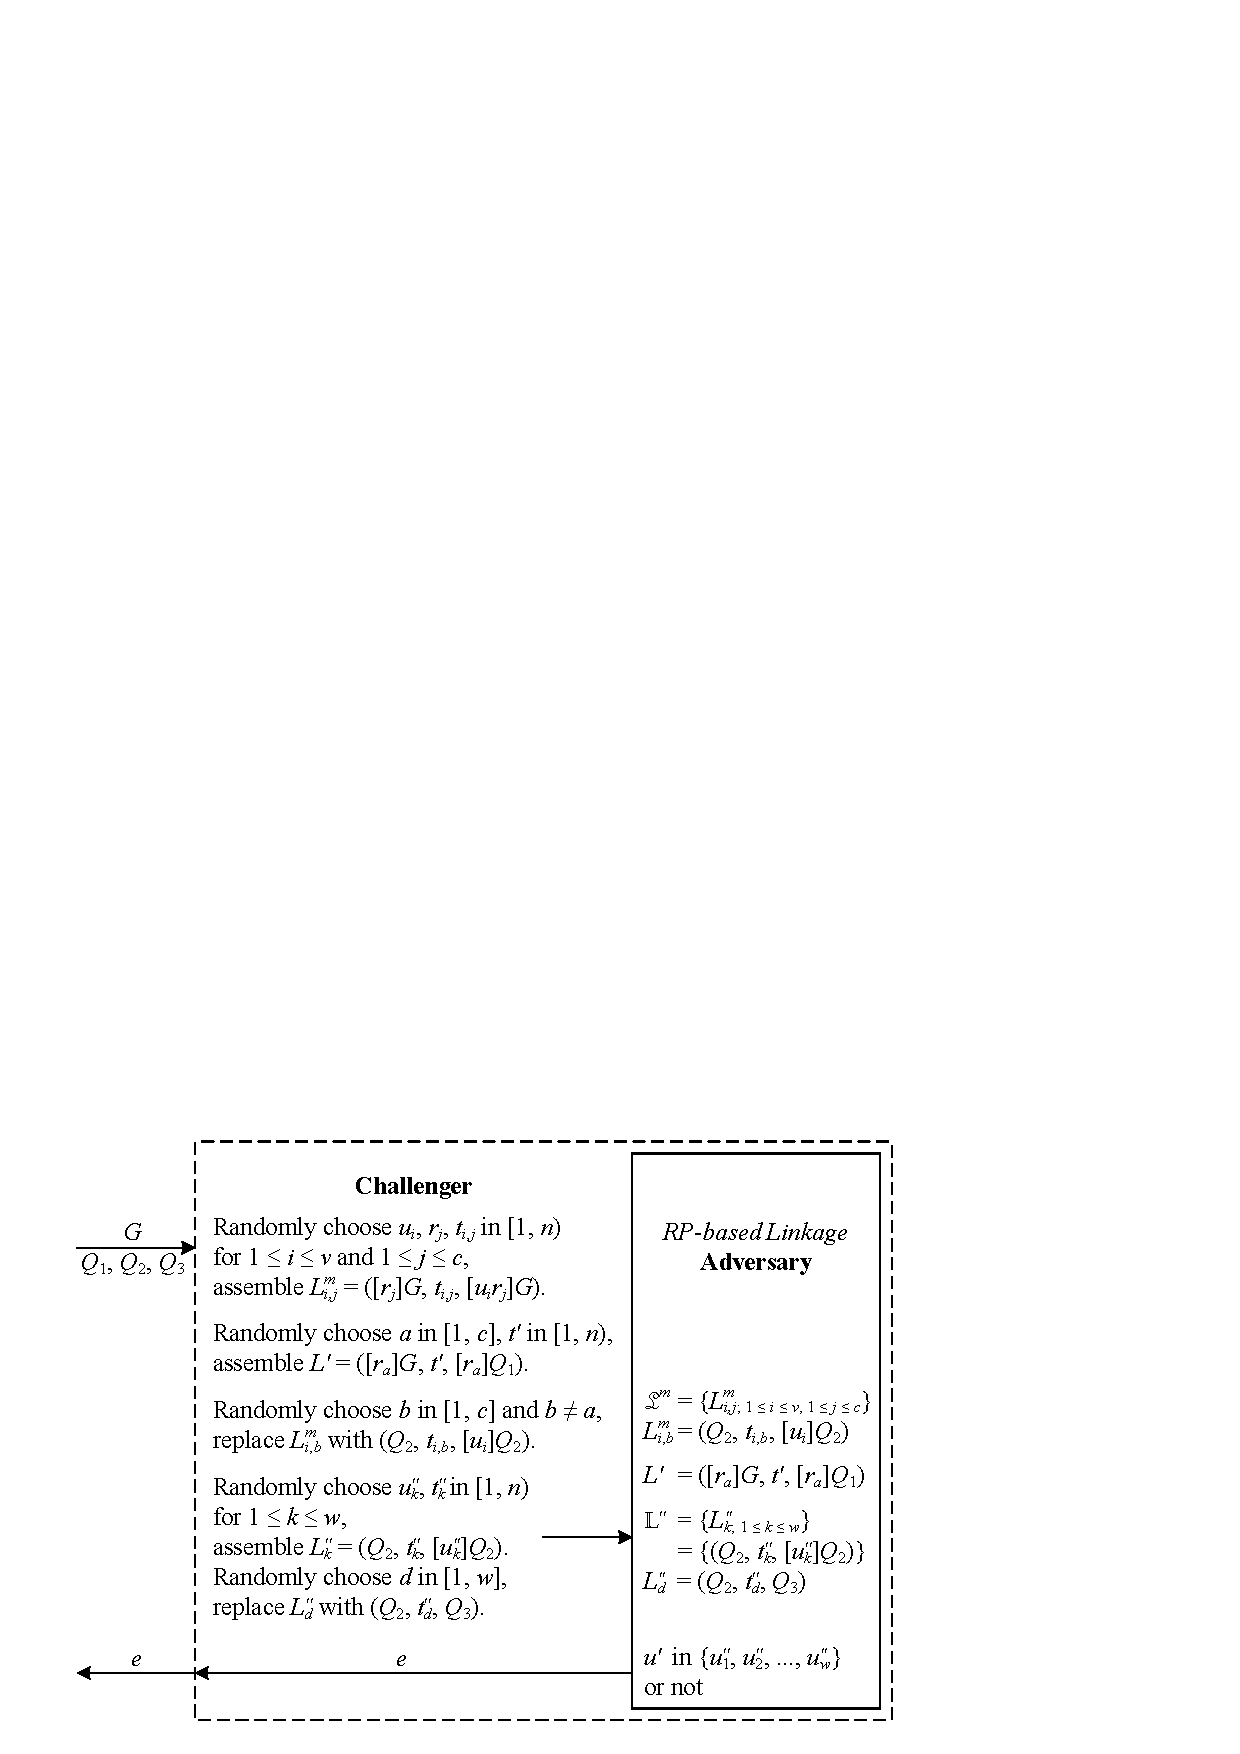
\includegraphics[width=1.0\linewidth]{fig/rp-linkage-game.pdf}
  \caption{The PPT algorithm $\mathcal{D}^*_R$ constructed based on the RP-based identity linkage game to solve the ECDDH problem.}
  \label{fig:dalgorithm}
\end{figure}


%\vspace{-0.5mm}
\begin{thm}[RP Unlinkability]
\emph{Given $\mathbbm{L}$ and $\mathfrak{L}^m$, $c$ RPs colluding with $v$ users cannot link any login visiting some of these RPs by an honest user to any subset of logins visiting any other RPs by honest users.}
\label{thm-rp-unlinkability}
\end{thm}
%\vspace{-0.5mm}

\noindent\textbf{\textsc{Proof.}} Out of $\mathbbm{L}$
 we randomly choose a login $L' \neq L^m_{i,j}$ $(1 \le i \le v, 1 \le j \le c)$,
 which is initiated by an (unknown) honest user with $ID_{U'}=u'$ to a malicious $RP_{a}$ where $a \in [1,c]$.
Then, we randomly choose another malicious $RP_{b}$, where $b \in [1,c]$ and $b \neq a$.
Consider any subset $\mathbbm{L}'' \subset \mathbbm{L}$ of $w$ $(1 \leq w < s-v)$ logins visiting $RP_{b}$ by unknown honest users,
 and denote the identities of the users initiating these logins as $\mathbbm{u}_w=\{{u''_1}, {u''_2}, \cdots, {u''_w}\} \subset \mathbbm{u}$.

Next, we prove that the colluding adversaries cannot distinguish $u' \in \mathbbm{u}_w$ from $u'$ randomly selected in the universal set (i.e., $u' \in \mathbb{Z}_n$).
This indicates the adversaries cannot link $L'$ to another login (or a subset of logins) visiting $RP_{b}$.


We define an RP-based identity linkage game $\mathcal{G}_R$ between an adversary and a challenger, to describe this login linkage: the adversary receives $\mathfrak{L}^m$, $L'$, and $\mathbbm{L}''$ from the challenger and outputs $e$, where (\emph{a}) $e = 1$ if it decides $u'$ is in $\mathbbm{u}_w$ %$\{{U''_1}, {U''_2}, \cdots, {U''_w}\}$
or (\emph{b}) $e=0$ if it believes $u'$ is randomly chosen from $\mathbb{Z}_n$.
Thus, the adversary succeeds in $\mathcal{G}_R$ with an advantage $\mathbf{Adv}$:
\begin{align*}
&{\rm Pr}_1={\rm Pr}(\mathcal{G}_R(\mathfrak{L}^m, L', \mathbbm{L}'')=1 \;| \; u' \in \mathbbm{u}_w)  \\
&{\rm Pr}_2={\rm Pr}(\mathcal{G}_R(\mathfrak{L}^m, L', \mathbbm{L}'')=1 \; | \; u' \in \mathbb{Z}_n)\\
&{\mathbf{Adv}}=|{\rm Pr}_1-{\rm Pr}_2|
\end{align*}

As depicted in Figure \ref{fig:dalgorithm}, we then design a PPT algorithm $\mathcal{D}^*_R$ based on $\mathcal{G}_R$ to solve the elliptic curve decisional Diffie-Hellman (ECDDH) problem: given $(G, [x]G$, $[y]G$, $[z]G)$, decide whether $z$ is equal to $xy$ or randomly chosen in $\mathbb{Z}_n$, where $G$ is a point on an elliptic curve $\mathbb{E}$ of order $n$, and $x$ and $y$ are integers randomly and independently chosen in $\mathbb{Z}_n$.


The algorithm $\mathcal{D}^*_R$ works as follows. (1) On receiving an input $(G, Q_1=[x]G, Q_2=[y]G, Q_3=[z]G)$,
the challenger
chooses random numbers in $\mathbb{Z}_n$ to construct $\{u_i\}$, $\{r_j\}$, and $\{t_{i, j}\}$ for $1 \le i \le v$ and $1 \le j \le c$, with which it assembles $L^m_{i, j}=([r_j]G, t_{i,j}, [u_ir_j]G)$.
It ensures $[r_{j}]G \neq Q_2$ (or $r_j \neq y$) in this procedure.
(2) It randomly chooses $a \in [1, c]$ and $t' \in \mathbb{Z}_n$, to assemble $L' = ([r_{a}]G, t', [r_{a}]Q_1) = ([r_{a}]G, t', [xr_{a}]G)$.
(3)
Next, the challenger randomly chooses $b \in [1, c]$ but $b \neq a$, and replaces $ID_{RP_b}$ with $Q_2 = [y]G$.
Hence, for $1 \le i \le v$, the challenger replaces $L^m_{i, b}=([r_b]G, t_{i,b}, [u_ir_b]G)$ with $(Q_2, t_{i,b}, [u_i]Q_2) = ([y]G, t_{i,b}, [u_iy]G)$, and finally constructs $\mathfrak{L}^m$.
(4) The challenger chooses random numbers in $\mathbb{Z}_n$ to construct $\{u''_k\}$ and $\{t''_k\}$ for $1 \leq k \leq w$,
 with which it assembles $\mathbbm{L}'' = \{L''_{k; 1\leq k \leq w}\} = \{(Q_2, t''_k, [u''_k]Q_2)\} = \{([y]G, t''_k, [u''_ky]G)\}$.
It ensures $[u''_k]G \neq Q_1$ (i.e., $u''_k \neq x$) and $u''_k \neq u_i$,
 for $1 \le i \le v$ and $1 \le k \le w$.
Finally, it randomly chooses $d \in [1, w]$ and replaces $L''_{d}$ with $(Q_2, t''_d, Q_3) = ([y]G, t''_d, [z]G)$.
 Thus, $\mathbbm{L}'' = \{L''_{k;1\leq k \leq w}\}$ represents the logins initiated by $w$ honest users, i.e., $\mathbbm{u}_w=\{u''_1, u''_2, \cdots, u''_{d-1}, z/y, u''_{d+1}, \cdots, u''_w\}$.
 (5) When the adversary of $\mathcal{G}_R$ receives $\mathfrak{L}^m$, $L'$, and $\mathbbm{L}''$ from the challenger, it returns $e$ which is also the output of $\mathcal{D}^*_R$.

According to the above construction, % of $\mathfrak{L}$, $L'$ and $\mathbbm{L}''$,
$x$ is embedded as $ID_{U'}$ of the login $L'$ visiting the RP with $ID_{RP_{a}} = [r_{a}]G$,
and $z/y$ is embedded as $ID_{U''_d}$ of $\mathbbm{L}''$ visiting the RP with $ID_{RP_{b}}=[y]G$,
together with $\{u''_1, \cdots, u''_{d-1}, u''_{d+1}, \cdots, u''_w\}$.
Meanwhile, $[r_{a}]G$ and $[y]G$ are two malicious RPs' identities in $\mathfrak{L}^m$.
Because $x \neq u''_{k; 1\leq k \leq w, k \neq d}$ and then $x$ is not in $\{u''_1, \cdots, u''_{d-1}, u''_{d+1}, \cdots, u''_w\}$, the adversary outputs $s=1$ and succeeds in the game \emph{only if} $x = z/y$.
Therefore, using $\mathcal{D}^*_R$ to solve the ECDDH problem, we have an advantage $\mathbf{Adv}^*=|{\rm Pr}^*_1 - {\rm Pr}^*_2|$, where
\begin{align*}
&{\rm Pr}^*_1 =  {\rm Pr}(\mathcal{D}^*_R(G, [x]G, [y]G, [xy]G)=1) \\
=&{\rm Pr}(\mathcal{G}_R(\mathfrak{L}^m, L', \mathbbm{L}'')=1 \; | \; u' \in \mathbbm{u}_w) = {\rm Pr}_1 \\
&{\rm Pr}^*_2= {\rm Pr}(\mathcal{D}^*_R(G, [x]G, [y]G, [z]G)=1) \\
=&{\rm Pr}(\mathcal{G}_R(\mathfrak{L}^m, L', \mathbbm{L}'')=1 \; | \; u' \in \mathbb{Z}_n) = {\rm Pr}_2 \\
&\mathbf{Adv}^*=|{\rm Pr}^*_1-{\rm Pr}^*_2|=|{\rm Pr}_1-{\rm Pr}_2|={\mathbf{Adv}}
\end{align*}

If in $\mathcal{G}_R$ the adversary has a non-negligible advantage, then $\mathbf{Adv}^*={\mathbf{Adv}}$ is also non-negligible regardless of the security parameter $\lambda$. This violates the ECDDH assumption.

Therefore, the adversary has no advantage in $\mathcal{G}_R$ and cannot decide whether $L'$ is initiated by some honest user with an identity in $\mathbbm{u}_w$ or not.
Because $RP_b$ is any malicious RP, this proof can be easily extended from $RP_b$ to more colluding malicious RPs.
\hfill $\square$


\subsection{Account Synchronization}
\label{account-syn}
If new users are allowed to register after the initialization,
in order to distinguish meaningful accounts from meaningless ones in Step 3.3,
 an RP needs to regularly synchronize its accounts from the IdP.
For example,
    when an account is derived but not in the visited RP's local account list,
        the RP contacts the IdP to synchronize accounts.
Then, after the instant account synchronization, 
    the token holder will be rejected
     if the derived account is still considered as meaningless (i.e., not in the RP's local account list).

An RP cannot imperceptively treat the token holder with an account not in the list
 as a newly-registered user.
Although a malicious user cannot log into this RP as any meaningful account belonging to other users according to Theorems \ref{thm-u-id} and \ref{thm-rp-designation},
 she could log into such an RP as a meaningless but identical account in multiple logins.
For example, both $\hat{t}$ and $\check{t}$ ($\check{t} \neq \hat{t}$) are reused in these logins,
    as analyzed in the proof of Theorem \ref{thm-u-id}.
Then, this malicious user actually owns multiple accounts at one RP.
%\footnote{In this case, $\hat{t}$ and $\check{t}$ are long-term secrets kept by the malicious user, and $\check{t}$ is sent to the RP. For such a malicious user, the system actually provides services of identity federation. Then, even when the IdP is colluding with RPs, the ``meaningless'' accounts belong to this user across RPs cannot be linked because $\hat{t}$ masks the relationship among these accounts.}


The instant account synchronization can be replaced by conditional $PID_{RP}$ checking as below.
If an RP derives some account not in its local account list,
    it additionally checks $PID_{RP}$ in this case:
     If $PID_{RP}$ enclosed in the signed token is equal to $[t]ID_{RP}$,
                this account is asserted to belong to a newly-registered user\footnote{In this case, adversaries cannot manipulate $t$ and then the derived account is meaningful.}
                and the RP updates its account list locally;
    otherwise, it rejects this token.


